\documentclass[twoside, 10pt]{article}

\usepackage{geometry}
\geometry{outer=2em, inner=2.2cm, top=6em, bottom=4em, headheight=\paperheight}
\usepackage[export]{adjustbox}
\usepackage{array}
\usepackage{amsmath}
\usepackage{amsfonts}
\usepackage{fancyhdr}
\pagestyle{fancy}
\fancyhf{}
\lhead{Algebra II - BASE}
\chead{Function  Characteristics - Business Applications}
\rhead{Practice, Page \thepage}
\usepackage{lastpage}
\usepackage{xcolor}
\usepackage{enumitem}
\usepackage{pifont}
\usepackage{graphicx}
\graphicspath{{../img}}
\usepackage{pgfplots}
\pgfplotsset{compat=1.18}
\usepackage{tabularx}
\usepackage{tikz}
\usetikzlibrary{patterns}

\newcommand{\R}{\mathbb R}
\newcommand{\e}{{\rm e}}
\newcommand{\pobr}[1]{\left\langle#1\right\rangle}
\newcommand{\norm}[1]{\lVert #1 \rVert}
\newcommand{\abs}[1]{\lvert #1 \rvert}

\DeclareMathOperator{\xd}{d\!}
\DeclareMathOperator{\proj}{proj}

\title{}
\date{}

\begin{document}
\noindent
{\large
First Name \rule{6em}{.1pt}\hspace{\stretch{1}}Last Name \rule{6em}{.1pt}\hspace{\stretch{1}} Date \rule{1.5em}{.1pt} -- \rule{1.5em}{.1pt} -- \rule{1.5em}{.1pt}\hspace{\stretch{1}} Period \rule{2em}{.1pt}\hspace{\stretch{1}} Score \rule{2em}{.1pt}
}
\vspace{1em}

{\noindent \bf Learning Objectives.}
\begin{itemize}
\item
Use the profit-price graph to make informed business decisions.
\end{itemize}
{\noindent\bf Discussion.}

Suppose you own or manage a business. Setting the price for your product is one of the most nuanced decisions you will make. Discuss the prompts below with your classmates for 5 minutes and write a brief summary for each prompt.

\begin{itemize}
\item
How might raising the price of a product affect the number of units sold?
\vspace{\stretch{1}}
\item 
Can raising the price always increase profit?
\vspace{\stretch{1}}
\item 
What trade-offs do businesses face when setting prices?
\vspace{\stretch{1}}
\item As a business decision-maker, what principles will you follow when setting prices to benefit the business?
\vspace{\stretch{1}}
\end{itemize}

{\noindent\bf Problems.}

The grunt work has been completed. Your colleagues in market research and sales operations have collected the data, performed the calculations, and developed the following profit-price model (function): the profit, $p(x)$, in hundreds of dollars, as a function of the unit price, $x$, in tens of dollars, is given below
\[
p(x) = -3x^2 + 13.2x-6.8
\]
Now, as the decision maker, examine the model and choose the option that best serves your business.
Answer the following questions according to this model.
\begin{enumerate}[leftmargin=*]
\item Determine if \((2, 7.5)\) and \((2, 7.6)\) are on the graph of the function rigorously. Show your justification work below. 
\vspace{\stretch{1}}
\item Given  \((1, 3.4)\) and \((4, -2)\) are two points on the graph, interpret the meaning of them in business language. (Hint: Be mindful of the units!)
\vspace{\stretch{1}}
\clearpage
\item What does ``break even'' mean? What should a break even point look like on the graph of the function?
\vspace{\stretch{1}}

\begin{center}
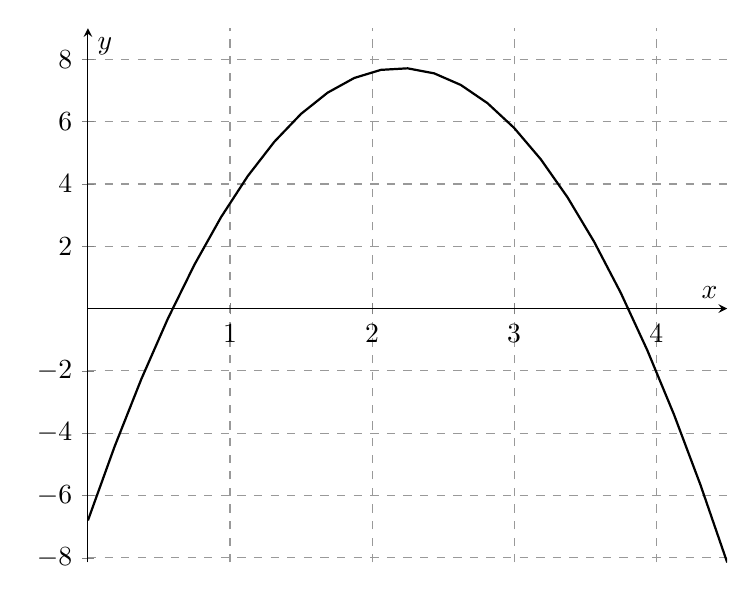
\begin{tikzpicture}
\begin{axis}[
axis lines=middle,
ymax=9,
domain=0:4.5,
ytick distance=2,
grid=both,
grid style={draw=gray!80, dashed},
xlabel={$x$},
ylabel={$y$},
width=0.8\textwidth,
]
\addplot[thick]{-3*x^2 + 13.2*x-6.8};
\end{axis}
\end{tikzpicture}
\end{center}
\item According to the graph of the function, what is the break even price of the business?
\vspace{\stretch{1}}

\item What is the price that produces the maximum profit for the business?
\vspace{\stretch{1}}
\end{enumerate}

\end{document}